\section{卷积神经网络}
\subsection{模型的结构}
卷积神经网络是一种由卷积层、池化层、全连接层等模块组成的一种人工神经网络。其中,卷积层会使用多个卷积核对输入张量进行卷积操作,并输出通道数等于卷积核数量的特征图,特别的,对于$1\times 1$卷积,相当于在每个像素的通道维度上做全连接;池化层会通过某种方式(如最大值、平均值)等对输入张量进行下采样,缩小输入的维度;而全连接层则为多层感知机(MLP)网络,对输入张量进行全连接,最后的输出向量可用于分类、回归等任务。在图像超分辨率这一领域中,卷积神经网络中一般不使用全连接层,而是直接输出一张结果图像。如图\ref{fig:SRCNN}是SRCNN模型的结构,输入图像首先双三次上采样到期望的尺寸,然后经过一个卷积核尺寸$9\times 9$,拥有64个卷积核的卷积层,输出一个64通道的特征图;再经过一个卷积核尺寸$1\times 1$,拥有32个卷积核的卷积层,输出一个32通道的特征图;最后经过一个卷积核尺寸$5\times 5$,拥有3个卷积核的卷积层,输出一个3通道的特征图,而此输出则为最终生成的高分辨率图像。
\subsection{模型的训练和推理}
对于简单的卷积神经网络如SRCNN,可以使用监督式训练。训练过程中,输入batch中会包含成对的高分辨率和低分辨率图像。网络输入低分辨率图像,输出超分图像,用超分图像和高分辨率图像计算均方差损失函数(MSE Loss),随后使用随机梯度下降(SGD)等优化器对模型参数进行优化,经过若干次迭代,直到损失函数收敛。在推理时,只需要输入低分辨率图像,即可使用训练好的模型生成超分图像。

\begin{figure}[htbp]
    \centering
    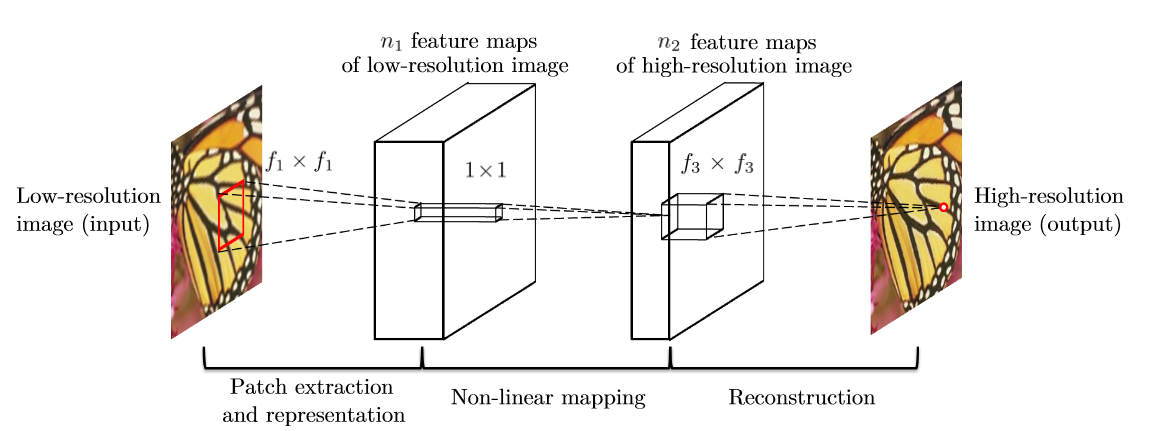
\includegraphics[width=1.0\textwidth]{imgs/SRCNN.png}
    \caption{SRCNN的结构}
    \label{fig:SRCNN}
\end{figure}

\section{基于无监督学习的超分辨率模型}

\section{不确定性学习}
